%% TCDimerTreeTopology
%% FigTCDimerTreeTopologyBiophysical.tex
%% Unused packages and definitions removed; TikZ/PGFPlots source formatted.

\documentclass[tikz,margin=2mm]{standalone}
\usetikzlibrary{arrows}

\def\half{\frac{1}{2}}

\def\KG{K_G}
\def\KL{K_L}

\def\L{{\rm L}}
\def\G{{\rm G}}
\def\R{{\rm R}}
\def\LR{{\rm L}{\rm R}}
\def\RG{{\rm R}{\rm G}}
\def\LRG{{\rm L}{\rm R}{\rm G}}

\begin{document}

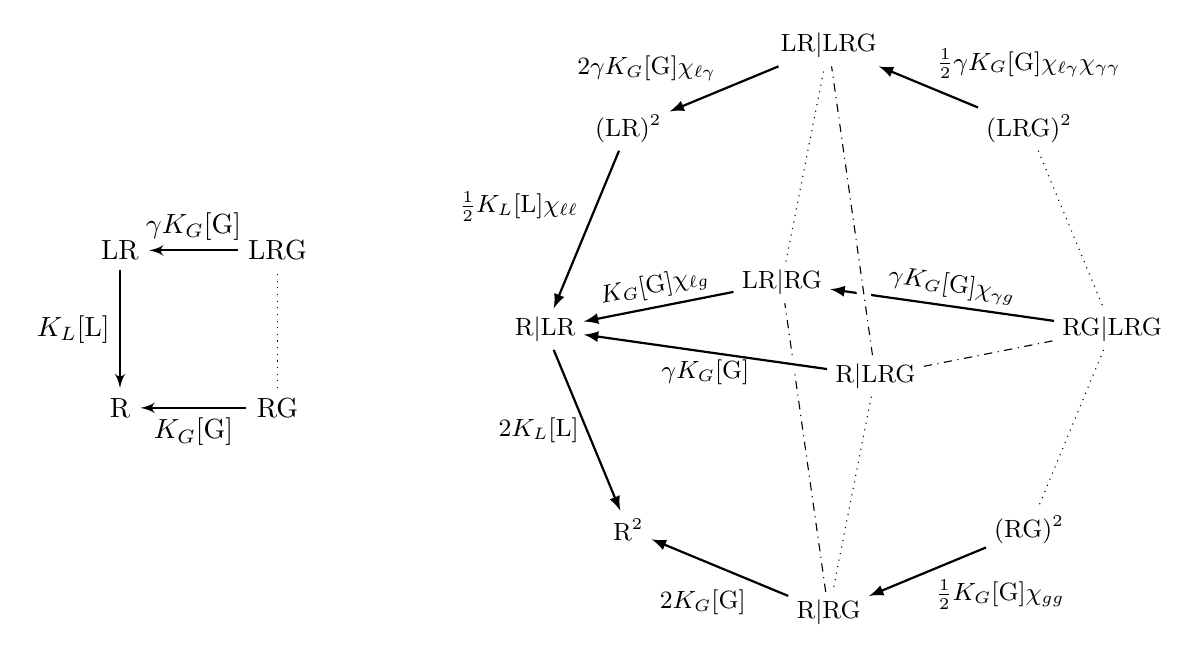
\begin{tikzpicture}[scale=1,style=thick,shorten >=0pt,shorten <=0pt,>=latex']

    %\begin{scope}[node distance=1.4cm,xshift=-6cm,yshift=2.7cm]
        %\node (B) {$a_2$};
        %\node[below of = B] (A) {$a_1$};
        %\draw [->,thick] (B) to node[left,align=center] {$e_2$} (A);
        %\node[right of = A] (C) {$a_3$};
        %\draw [<-,thick] (A) to node[below] {$e_3$} (C);
        %\node[right of = B] (D) {$a_4$};
        %\draw [->,thick] (D) to node[below] {$e_4$} (B);
        %\path (B) to node[above,yshift=0.5cm] {$T \subset H $:} (D);
        %\draw [dotted,thin] (C) to (D);
        %\end{scope}

    %\begin{scope}[xshift=8cm,yshift=3cm,node distance=2cm,>=latex',font=\small]
        %\node (LR) {$\LR$};
        %\node[below of = LR] (R) {$\R$};
        %\draw [left to-,thick,transform canvas={xshift=-1.5pt}] (LR) to node[left] {$\KL$} (R);
        %\draw [dashed,left to-,thick,transform canvas={xshift=1.5pt}] (R) to  (LR) ;
        %\node[right of = R] (RG) {$\RG$};
        %\draw [-right to,thick,transform canvas={yshift=-1.5pt}] (R) to node[below] {$\KG$} (RG);
        %\draw [dashed,-right to,thick,transform canvas={yshift=1.5pt}] (RG) to (R);
        %\node[right of = LR] (LRG) {$\LRG$};
        %\draw [dashed,right to-,thick,transform canvas={xshift=-1.5pt}] (RG) to (LRG);
        %\draw [right to-,thick,transform canvas={xshift=1.5pt}] (LRG) to node[right] {$\gamma \KL$} (RG) ;
        %\draw [dashed,left to-,thick,transform canvas={yshift=-1.5pt}] (LR) to (LRG);
        %\draw [left to-,thick,transform canvas={yshift=1.5pt}] (LRG) to node[above] {$\gamma \KG$} (LR);
        %\end{scope}

    \begin{scope}[node distance=2cm,xshift=8cm,yshift=1cm]
        \node (B) {$\LR$};
        \node[below of=B] (A) {$\R$};
        \draw[->,thick] (B) to node[left,align=center] {$\KL [\L]$} (A);
        \node[right of=A] (C) {$\RG$};
        \draw[<-,thick] (A) to node[below] {$\KG [\G]$} (C);
        \node[right of=B] (D) {$\LRG$};
        \draw[->,thick] (D) to node[above] {$\gamma \KG [\G]$} (B);
        \draw[dotted,thin] (C) to (D);
        %\path (B) to node[above,yshift=1cm] {$T(H)$} (D);
    \end{scope}

    %\begin{scope}[xshift=0cm,yshift=0cm,scale=1,shorten >=0pt,shorten <=0pt]
        %\coordinate (title) at (90:4);
        %\draw (title) node {$[T(H)]^{(2)} \subset H^{(2)}$};
        %\draw (0:3) node[] (cd) {$cd$};
        %\draw (45:3) node[] (d2) {$d^2$};
        %\draw (90:3) node[] (bd) {$bd$};
        %\draw (135:3) node[] (b2) {$b^2$};
        %\draw (180:3) node[] (ab) {$ab$};
        %\draw (225:3) node[] (a2) {$a^2$};
        %\draw (270:3) node[] (ac) {$ac$};
        %\draw (315:3) node[] (c2) {$c^2$};
        %\draw (315:0.7) node[] (ad) {$ad$};
        %\draw (135:0.7) node[] (bc) {$bc$};
        %\draw[<-,thick] (a2) -- node[left] {$2\kappab[a]$} (ab);
        %\draw[<-,thick] (ab) -- node[above left] {$\frac{1}{2}\kappab[b]$} (b2);
        %\draw[<-,thick] (b2) --  node[pos=0.75] (b2bd) {} node[above left] {$2\kappad[b]$} (bd);
        %\draw[<-,thick] (bd) -- node[above right] {$\frac{1}{2}\kappad[d] $} (d2);
        %\draw[thin,dotted] (d2) -- (cd);
        %\draw[thin,dotted] (cd) -- (c2);
        %\draw[<-,thick] (ac) -- node[below right] {$\frac{1}{2}\kappac [c]$} (c2);
        %\draw[->,thick] (ac) -- node[below left] {$2\kappac[a]$} (a2);
        %\draw[thin,dotted] (bc) -- (bd);
        %\draw[thin,dotted] (ad) -- (ac);
        %\draw[<-,thick] (ab) --  node[above,sloped] {$\kappac[b]$} (bc);
        %\draw[<-,thick] (bc) -- node[above,sloped] {$\kappad[c] $} (cd);
        %%\draw[thin,dashdotted] (ad) --  (cd);
        %\draw[<-,thick] (ad) -- node[below,pos=0.5]  {$\kappac[d]$}  (cd);
        %%\draw[thin,dashdotted] (ad) -- node[pos=0.75] (adbd) {} (bd);
        %\draw[white,line width=5pt] (ad) -- node[pos=0.75] (adbd) {} (bd);
        %\draw[<-,thick] (ad) -- node[pos=0.65,right] (adbd) {$\kappab[d]$} (bd);
        %%\draw[thin,dashdotted] (ac) -- node[pos=0.75] (bcac) {} (bc);
        %\draw[<-, thick] (ac) -- node[left,pos=0.4] (bcac) {$\kappab[c]$} (bc);
        %\draw[white,line width=5pt] (ab) -- node[below] {$\kappad[a]$} (ad) ;
        %\draw[<-,thick] (ab) -- node[below] {$\kappad[a]$} (ad) ;
        %\end{scope}
    %
    %\begin{scope}[xshift=8cm,yshift=0cm,scale=1,shorten >=0pt,shorten <=0pt,outer sep=1pt,inner sep=2pt,>=latex]
        %\coordinate (title) at (90:4);
        %\draw (title) node {$\Theta(H^{(2)}) \subset [T(H)]^{(2)}$};
        %\draw (0:3) node[] (cd) {$cd$};
        %\draw (45:3) node[] (d2) {$d^2$};
        %\draw (90:3) node[] (bd) {$bd$};
        %\draw (135:3) node[] (b2) {$b^2$};
        %\draw (180:3) node[] (ab) {$ab$};
        %\draw (225:3) node[] (a2) {$a^2$};
        %\draw (270:3) node[] (ac) {$ac$};
        %\draw (315:3) node[] (c2) {$c^2$};
        %\draw (315:0.7) node[] (ad) {$ad$};
        %\draw (135:0.7) node[] (bc) {$bc$};
        %\draw[<-,thick] (a2) -- node[left] {$2\kappab$} (ab);
        %\draw[<-,thick] (ab) -- node[above left] {$\frac{1}{2}\kappab\etabb$} (b2);
        %\draw[<-,thick] (b2) --  node[pos=0.75] (b2bd) {} node[above left] {$2\kappad\etabd$} (bd);
        %\draw[<-,thick] (bd) -- node[above right] {$\frac{1}{2}\kappad \etabd\etadd$} (d2);
        %%\draw[thin,dotted] (d2) -- (cd);
        %%\draw[thin,dotted] (cd) -- (c2);
        %\draw[<-,thick] (ac) -- node[below right] {$\frac{1}{2}\kappac \etacc $} (c2);
        %\draw[->,thick] (ac) -- node[below] {$2\kappac$} (a2);
        %%\draw[thin,dotted] (bc) -- (bd);
        %
        %%\draw[thin,dotted] (ad) -- (ac);
        %\draw[thin,dashdotted] (ac) -- node[pos=0.75] (bcac) {} (bc);
        %\draw[<-,thick] (ab) --  node[above,sloped] {$\kappac \etabc$} (bc);
        %\draw[<-,thick] (bc) -- node[above,sloped] {$\kappad \etacd$} (cd);
        %\draw[thin,dashdotted] (ad) --  (cd);
        %
        %\draw[white,line width=5pt] (ab) -- node[below] {} (ad) ;
        %\draw[<-,thick] (ab) -- node[below] {$\kappad$} (ad) ;
        %
        %\draw[white,line width=5pt] (ad) -- node[pos=0.75] (adbd) {} (bd);
        %\draw[thin,dashdotted] (ad) -- node[pos=0.75] (adbd) {} (bd);
        %\end{scope}

    \begin{scope}[xshift=17cm,scale=1.2,shorten >=0pt,shorten <=0pt,outer sep=1pt,inner sep=2pt,>=latex,font=\small]
        %\coordinate (title) at (90:4);
        %\draw (title) node[font=\large] { biophysical notation};
        \draw (0:3) node[] (cd) {$\RG|\LRG$};
        \draw (45:3) node[] (d2) {$(\LRG)^2$};
        \draw (90:3) node[] (bd) {$\LR|\LRG$};
        \draw (135:3) node[] (b2) {$(\LR)^2$};
        \draw (180:3) node[] (ab) {$\R|\LR$};
        \draw (225:3) node[] (a2) {$\R^2$};
        \draw (270:3) node[] (ac) {$\R|\RG$};
        \draw (315:3) node[] (c2) {$(\RG)^2$};
        \draw (315:0.7) node[] (ad) {$\R|\LRG$};
        \draw (135:0.7) node[] (bc) {$\LR|\RG$};
        \draw[<-,thick] (a2) -- node[left] {$2K_L[\L]$} (ab);
        \draw[<-,thick] (ab) -- node[above left] {$\half K_L [\L] \chi_{\ell\ell}$} (b2);
        \draw[<-,thick] (b2) --  node[pos=0.75] (b2bd) {} node[above left] {$2 \gamma K_G [\G]\chi_{ \ell  \gamma } $} (bd);
        \draw[<-,thick] (bd) -- node[above right] {$\half \gamma K_G[\G] \chi_{\ell \gamma } \chi_{\gamma\gamma}$} (d2);
        \draw[thin,dotted] (d2) -- (cd);
        \draw[thin,dotted] (cd) -- (c2);
        \draw[<-,thick] (ac) -- node[below right] {$\half K_G [\G]\chi_{gg}$} (c2);
        \draw[->,thick] (ac) -- node[below left,pos=0.25] {$2K_G[\G]$} (a2);
        \draw[thin,dotted] (bc) -- (bd);

        \draw[thin,dotted] (ad) -- (ac);
        \draw[thin,dashdotted] (ac) -- node[pos=0.75] (bcac) {} (bc);  % dashdotted
        \draw[<-,thick] (ab) --  node[above,sloped] {$K_G [\G] \chi_{\ell g}$} (bc);
        \draw[<-,thick] (bc) -- node[above,sloped] {$\;\;\gamma K_G [\G]\chi_{\gamma g }$} (cd);
        \draw[thin,dashdotted] (ad) --  (cd);  % dashdotted

        \draw[white,line width=5pt] (ab) --  (ad);
        \draw[<-,thick] (ab) -- node[below] {$\gamma K_G [\G]$} (ad);

        \draw[white,line width=5pt] (ad) -- node[pos=0.75] (adbd) {} (bd);
        \draw[thin,dashdotted] (ad) -- node[pos=0.75] (adbd) {} (bd); % dashdotted

    \end{scope}

    %\draw (\left,\height) node[font=\large] {{\bf a}};
    %\draw (\left+8,\height) node[font=\large] {{\bf b}};
    %\draw (\left+16,\height) node[font=\large] {{\bf c}};

\end{tikzpicture}

\end{document}

